% !TeX root = ../main.tex
% Add the above to each chapter to make compiling the PDF easier in some editors.

\chapter{Related Works}\label{chapter:introduction}
In 3D multi-person human pose estimation, there are two challenging association problems in this task. First, it needs to associate the joints of the same person by either top-down or bottom-up strategies. Second, it needs to associate the 2D poses of the same person in different views based on appearance features which are unstable when people are occluded. We will show the pros and cons of both top-down and bottom-up approaches that tackle the mentioned association problems.
\section{Top-down Multi-person 3D Pose Estimation}
In top-down methods, humans are first detected, through bounding boxes, in
each view and 2D poses are estimated for each bounding box. Then, bounding boxes
are associated with individuals across multiple views. Next, estimated 2D poses are lifted to hypothesized 3D poses, where each individual might have more than one hypothesized 3D poses that need to be refined later. Finally, hypothesized 3D poses are refine, based on heuristic, 3DPS etc., to a single 3D pose for each individual.
\subsection{Single View}
 Rogez \textit{et al.} \cite{LCR2019} estimate multiple 3D humans poses with single-view natural images using the learning-based model. They cast the task of estimating multiple 3D human poses to a combination of classification and a regression problem. In their work, they store a set of anchor 2D-3D poses, denoted by $(\mathit{p}, \mathbf{P})$, that collected from the MoCap dataset. In their framework, an image is first fed into a localization network that outputs a set of bounding boxes, where each box $\mathit{B}$ contain a fixed set of predefined anchor poses with labels $\mathit{c_B} \in \{0 \dots K\}$ (0 is the background class). The scale of anchor poses is normalize according to the size of bounding boxes, making the regression independent of the scale and position of the person in the image. After the localization network is an RoI pooling layer and it is connected by two consecutive fully-connected networks: (1) \textit{pose classification network} and (2) \textit{pose regression network}. \textit{The classification network} aims at predicting the closest anchor-pose, i.e., the correct label, for each bounding box $\mathit{B}$. In other words, each bounding box $\mathit{B}$ is assigned with distribution $\mathit{u}$ among $\mathit{K}$ anchor poses plus background. \textit{The regression network} contains $\mathit{K+1}$ regressors, learned independently for each anchor pose. The regression outputs $\mathit{v}$, that has a dimension of $5 \times J \times (K+1)$ (5 because 2D + 3D coordinates) for each $\mathit{B}$ in one forward pass. See Fig. \ref{fig:ch3-overview-lcn} for the pipeline. The final 2D and 3D poses are the weighted averages on $\mathit{v}$ using the probability of anchor poses $\mathit{u}$.
 
 The advantage of this work is the network can outputs full 2D and 3D poses even when the humans are partially occluded. However, the diversity of the poses depending on the number of anchor poses. In addition, the optimization for reliable 2D and 3D poses from anchor poses is not convex.
 \begin{figure}
 	\centering
 	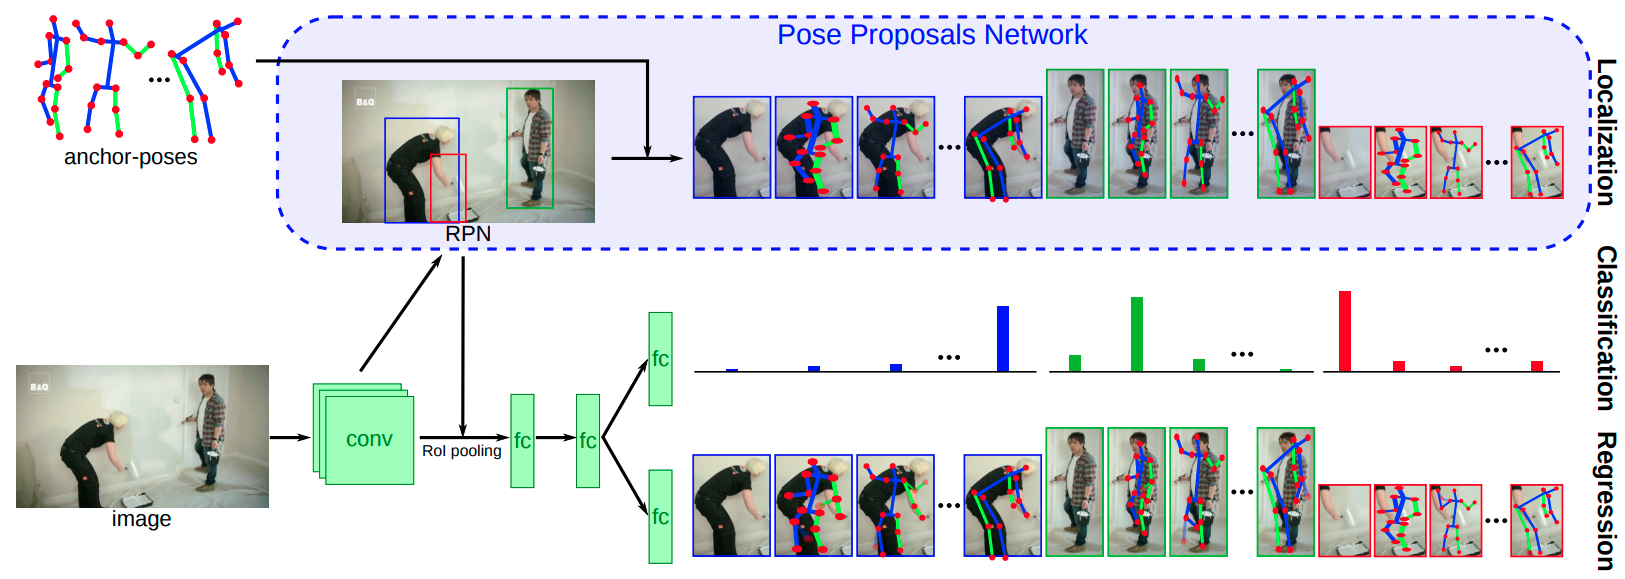
\includegraphics[width=1.0\columnwidth]{figures/ch3/overview-lcn.png}
 	\caption{Overview of the \cite{LCR2019} approach. It first extract candidate regions using a Region
 		Proposal Network (RPN) and obtain pose proposals by placing a fixed set of anchor-poses into these boxes (top). These pose proposals are then scored by a classification branch and refined using class-specific regressors, learned independently for each anchor-pose.} 
 	\label{fig:ch3-overview-lcn}
 \end{figure}
\subsection{Multiple Views}
Dong \textit{et al.} \cite{dong2019fast} first detects $\mathit{p_i}$ number of bounding boxes in \textit{i-th} view from an off-the-shelf 2D human pose detector \cite{Chen2018CPN}. To associate bounding boxes across views, they formulate the task as an optimization problem, that looks for an optimal permutation matrix $\mathbf{P}$ maximizes the corresponding affinities $\mathbf{A}$. Entries of the affinity matrix $\mathbf{A_{ij}} \in \mathbb{R}^{p_i \times p_j}$ are scores that composed by the appearance similarity and the geometric compatibility between bounding boxes. Specifically, the appearance scores are calculated from the euclidean distance between a pair of feature vectors, that generated by feeding the bounding boxes into a pre-trained re-ID model \cite{zhong2018camera}. Besides appearance,  another important cue to associate two bounding boxes is that their associated 2D poses should be geometric consistent. More specifically, the corresponding 2D joint locations should satisfy the epiplolar constraint (\ref{eq:epipolar-line}), i.e. a pair of corresponding joints should lie on the epipiolar lines associated with one and the other. Thus, the distance of joint 2D location $\mathbf{x_j}$, from \textit{j-th} view, should be as close as possible to the epipolar line $\mathit{L_{ij}}$ associated with $\mathbf{x_{i}}$ from the \textit{i-th} view and vice versa. While solving the optimal permutation matrix $\mathbf{P_{ij}}$ for maximizing $\langle \mathbf{P_{ij}, A_{ij}} \rangle$ between a pair of view can be done by Hungarian algorithm, when there are multiple views, solving the
matching problem separately for each pair of views ignores the cycle-consistency constraint and may lead to inconsistent results. The all-view permutation matrix $\mathbf{P}$, composed by $\mathbf{P_{ij}}$, is an optimal solution of $\langle P_{ij}, A_{ij} \rangle$ with cycle consistency condition \cite{cycle-consistency}. Finally, they solved 3D poses, from multiple hypothesized 3D poses estimated from paired 2D poses in different pairs of views, with 3DPS. As the number of views grows, however, the time complexity of using 3DPS to estimate 3D pose increases exponentially \cite{Chen_2020_CVPR}.

Chen \textit{et al.} \cite{Chen_2020_CVPR} formulate 3D human poses estimation as a tracking task across multiple views and timestamps. The approach has two stages: initialization and tracking stage. In tracking stage, given a pair of target (associated 2D and 3D poses in previous timestamps) and detection at the different time frames, they combine 2D and 3D geometric correspondences. For 2D correspondences, they use the euclidean distance between the 2D pose of target and detection as affinity measurements. For 3D correspondences, they back-project detection's 2D joint location to rays in 3-space and measures point-to-ray euclidean distance between target and detection. See Fig. \ref{fig:ch3-cheng}. When initialization, they use \cite{dong2019fast} approach. To estimate 3D poses, they use a weighted triangulation with a penalty rate depending on timestamps. Since they use only triangulation for estimating 3D poses, the approach can reach realtime and time complexity only grow linearly with the number of cameras.
\begin{figure}
	\centering
	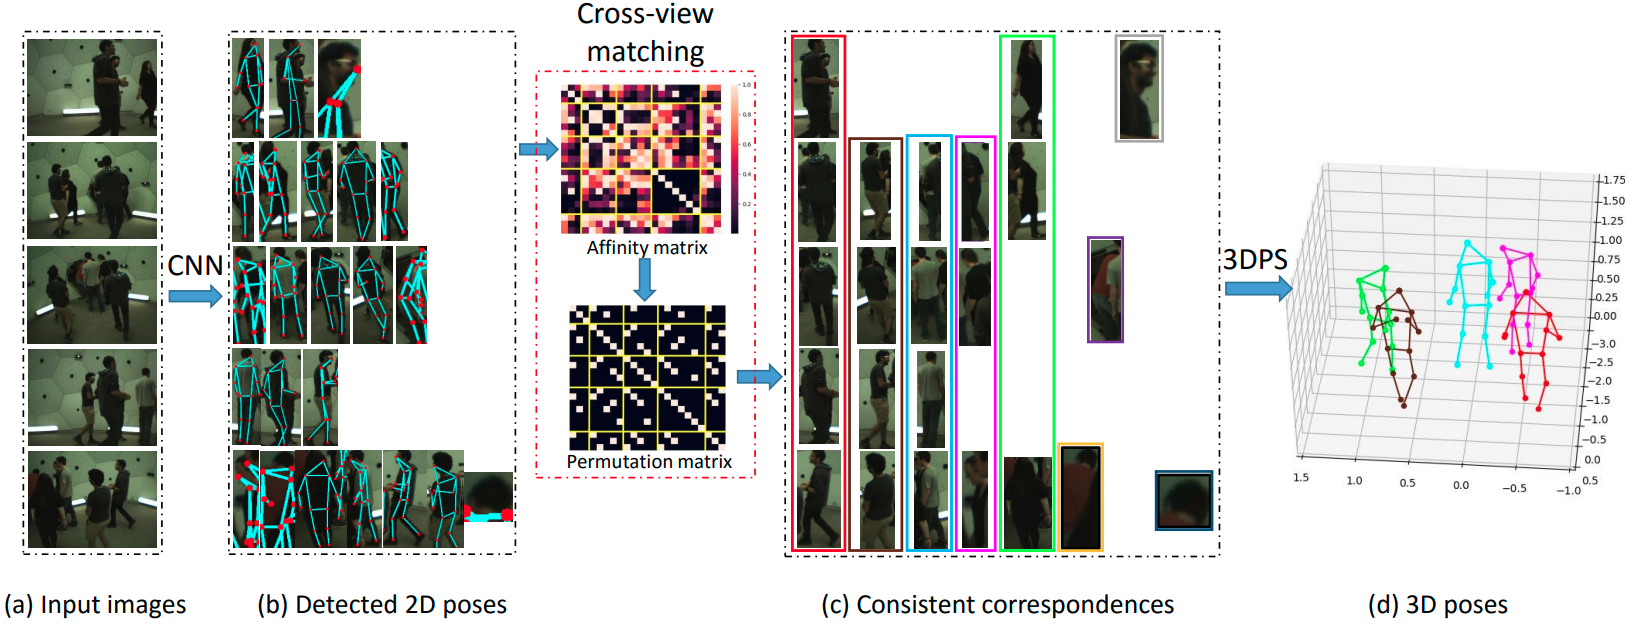
\includegraphics[width=0.7\columnwidth]{figures/ch3/dong-fast-cross-view-matching.png}
	\caption{Overview of the \cite{dong2019fast} approach. (a), an off-the-shelf human pose detector is used to produce 2D bounding boxes and associated 2D poses in each view, which may be inaccurate and incomplete (b). Then, the detected bounding boxes are clustered. Each resulting cluster includes the bounding boxes of the same person in different views (c). The isolated bounding boxes that have no matches in other views are regarded as false detections and discarded. Finally, the 3D pose of each person is reconstructed from the corresponding bounding boxes and associated 2D poses (d).} 
	\label{fig:ch3-dong-fast-cross-view-matching}
\end{figure}
\begin{figure}
	\centering
	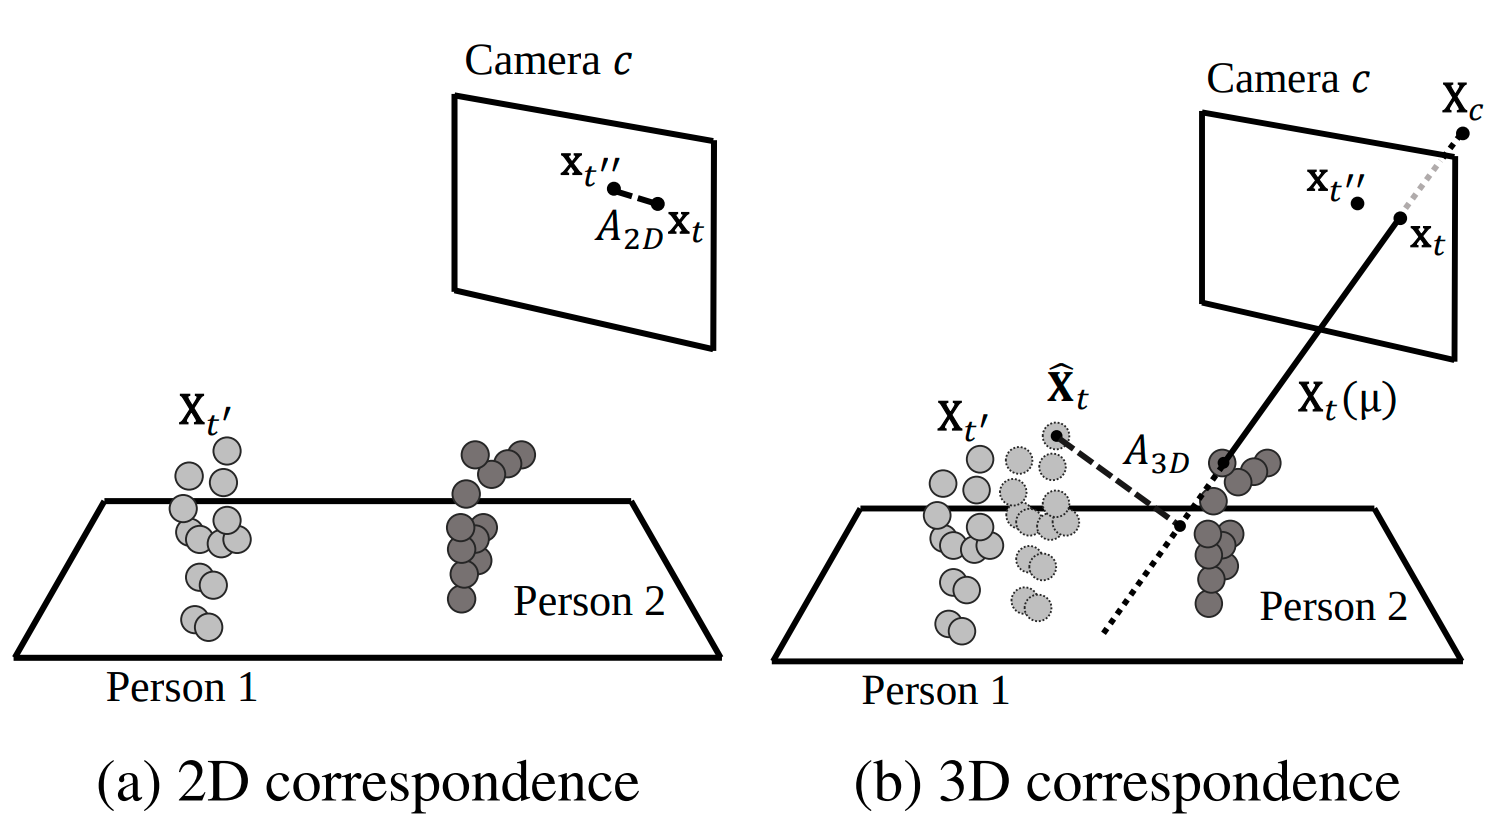
\includegraphics[width=0.7\columnwidth]{figures/ch3/chen-correspondence.png}
	\caption{2D and 3D correspondence affinity measurments in \cite{Chen_2020_CVPR}. Geometric affinity measurement. (a) 2D correspondence is computed within the same camera. (b) 3D correspondence is measured between the predicted location and the projected line in 3-space.} 
	\label{fig:ch3-cheng}
\end{figure}
\section{Bottom-up Multi-person 3D Pose Estimation}
In bottom-up methods, joints are estimated first and ,then, individuals are associated through some graph algorithms.
\subsection{Single View}
Metha \textit{et al.} \cite{singleshotmultiperson2018} regress the 3D coordinates of joints directly from a single-view image with DCNN. To tackle occlusion, they treat the rigid skeleton of the human body as a kinematic tree and embed 2D locations of sibling joints and root joint to the entries of feature maps called OPRM. Thus, joints are implicitly chained with siblings and the root joint. With the embedding, the DCNN learns not only how to predict 3D coordinate of joint but also the relation between joints while training on OPRM. To associate individuals, the DCNN predict part affinity field and joint heatmaps as well. To predict 3D coordinate of joints, they traverse the kinematic tree from root node, to get the base 3D pose, and from edge node, to get a more versatile 3D poses. The approach is able to reach real-time performance but the 3D poses suffers from error accumulation. In addition, the approach is not robust to occlusions , predicting unreliable 3D poses when two edge joints from different individuals are in proximity or occluded. 
\subsection{Multiple Views}
\cite{iskakov2019learnable, voxelpose} project 2D joint locations in all camera view into a common voxelized 3-space, where a projected 2D point become a ray in the voxelized 3-space. \cite{iskakov2019learnable, voxelpose} use 3D CNN to aggregate rays projected by same type of joints but from different views. Further, Tu \textit{et al.} \cite{voxelpose} use 3D CNN to predict cuboids that coarsely localize people, which can be consider as associating joints with individuals in 3-space with a learning-based method. See Fig. \ref{fig:ch3-overview-voxelpose}. The voxel-based approaches reach state-of-the-art, but these approaches require a fixed 3D grid that covers the whole environment. Thus, it only suits studio environments.

On one hand, approaches \cite{multiviewpose, epipolartransformers} propose to fuse joint heatmaps from multiple source views to a single reference view, solving occlusions issue by aggregate 2D joint predictions from other views and localize 2D joints as accurate as possible. Comparing with \cite{iskakov2019learnable, voxelpose}, these approaches does not work as good as voxel-based approach but are less computational demanding.
\begin{figure}
	\centering
	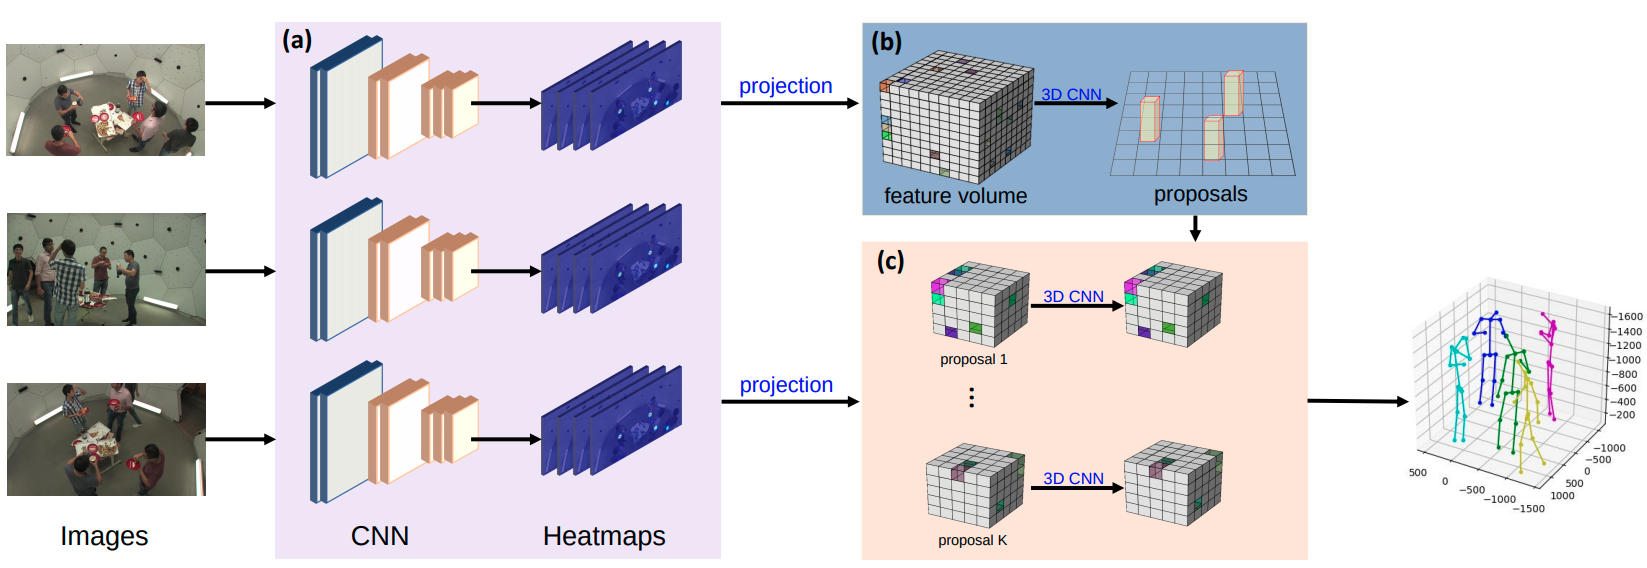
\includegraphics[width=1.0\columnwidth]{figures/ch3/overview-voxelpose.png}
	\caption{Overview of the \cite{voxelpose} approach. : (a) it first estimate 2D pose heatmaps for all views; then, (b) it warps the heatmaps to a common 3D space and construct a feature volume which is fed into a Cuboid Proposal Network to localize all people instances; (c) for each proposal, we construct a finer-grained feature volume and estimate a 3D pose.} 
	\label{fig:ch3-overview-voxelpose}
\end{figure}
\section{Temporal Fusion}
\cite{julieta2017motion, pavllo:videopose3d:2019} has shown that fusing 3D joints from multiple timestamps can help learning-based methods achieve better results. Since human motion is the result of both physical limitations (torque exerted by muscles, gravity,
moment preservation)) and the intentions of subjects, a learning-based method is able to pick these human motion dynamics to improve the smoothness of pose prediction. Pavllo \textit{et al.} \cite{pavllo:videopose3d:2019} use a ResNet-like architecture to estimate single-person 3D pose in YouTube video. The convolutional operation at each convolutional layer operate at temporal domain of the input. Moreover, the convolution kernel has dilation that increase with the depth of layer, drastically increasing the receptive field of hidden units at each layer. The residual connection connects neighboring layers between their inputs, so later layers have access to a higher temporal resolution from earlier layers. With only 4 layers, the hidden unit at output has a receptive field of 273 frames, generating temporal coherent single-person 3D pose from videos.

\section{Brief Conclusion}
In top-down approaches, the time complexity grows as number of people and view increased, since, in each view, human bounding boxes generates at least one 2D pose and bounding boxes needs to be associate with individuals across several views. On the contrary, ,in each view, bottom-up approaches estimate 2D locations of joints, by means of feature maps that has a fixed dimension regardless number of people in the view. Time complexity lies in the graph-based method or voxel-based method, which associating joints with individual across views. The voxel-based approaches suits only for constraint environments because it needs a dense 3D grid that cover the environments, refraining it from general applications. 
 
To this end, we briefly introduce our framework for multi-person 3D pose estimation can be divided into two parts: in the first stage, we trained our own 2D joint heatmap estimator that composed of several modules inspired by \cite{epipolartransformers, multiviewpose} multi-view fusion,  \cite{pavllo:videopose3d:2019} for temporal fusion. All the modules are fully convolutional and can be trained jointly. In the second stage, we associate 2D pose using \cite{tanke2019iterative}, a graph-based greedy method in associating 3D poses. Our framework is lightweight since it operate in 2D space and can be extended into an end-to-end training scheme.